% This is samplepaper.tex, a sample chapter demonstrating the
% LLNCS macro package for Springer Computer Science proceedings;
% Version 2.21 of 2022/01/12
%
\documentclass[runningheads]{llncs}
%
\usepackage[T1]{fontenc}
% T1 fonts will be used to generate the final print and online PDFs,
% so please use T1 fonts in your manuscript whenever possible.
% Other font encondings may result in incorrect characters.
%
\usepackage{graphicx}
% Used for displaying a sample figure. If possible, figure files should
% be included in EPS format.
%
% If you use the hyperref package, please uncomment the following two lines
% to display URLs in blue roman font according to Springer's eBook style:
%\usepackage{color}
%\renewcommand\UrlFont{\color{blue}\rmfamily}
%\urlstyle{rm}
%
\usepackage{orcidlink}
\usepackage{float}
\begin{document}
%
\title{Countermeasures in IoT Devices Using Reinforcement Learning}
%
%\titlerunning{Abbreviated paper title}
% If the paper title is too long for the running head, you can set
% an abbreviated paper title here
%
\author{C\'{e}sar {Rodr\'{i}guez~Villagr\'{a}}\inst{1}\orcidlink{0009-0007-0122-7417} \and Amanda P\'{e}rez Olmos \inst{1} \orcidlink{0009-0002-6157-5775} \and Rub\'{e}n Ruiz Gonz\'{a}lez\inst{1}\orcidlink{0000-0001-7006-2395} \and Nu{\~n}o Basurto\inst{1}\orcidlink{0000-0001-7289-4689}}
%
\authorrunning{C. Rodr\'{i}guez Villagr\'{a}.}
% First names are abbreviated in the running head.
% If there are more than two authors, 'et al.' is used.
%
\institute{Grupo de Inteligencia Computacional Aplicada (GICAP), Universidad de Burgos, \\
Av. Cantabria s/n, 09006 Burgos, Spain \\
\email{\{crv1002, apo1004\}@alu.ubu.es, \{ruben.ruiz, nbasurto\}@ubu.es}}
%
\maketitle              % typeset the header of the contribution
%
\begin{abstract}
Cybersecurity in IoT devices is crucial for ensuring continuous functionality and service availability. As these devices become more interconnected, they are becoming increasingly vulnerable to cyberattacks, particularly Denial-of-Service (DoS) and Distributed Denial-of-Service (DDoS) attacks, which have caused severe disruptions in recent years. These attacks can overload the network infrastructure, causing slow performance or total service failures. 
To address this issue, the implementation of a reinforcement learning (RL) agent within the network router is proposed to intelligently detect and mitigate DoS and DDoS attacks in real-time. Unlike traditional rule-based security mechanisms, RL agents dynamically adapt to evolving attack patterns, making them more effective against sophisticated threats. The agent learns to identify malicious traffic by attempting to saturate the queue and discard it, preventing network congestion and ensuring stable performance.
The key objective of this approach is to minimize packet loss while maintaining high network efficiency. The experimental results demonstrate that the proposed system effectively reduces the impact of DoS and DDoS attacks, strengthening the resilience of IoT networks against cyber threats.

 

\keywords{Internet of Things \and Security \and Reinforcement learning.}
\end{abstract}
%
%
%
\section{Introduction}

The rapid growth of the Internet of Things (IoT) has introduced new challenges for ensuring the security of networked devices. As IoT devices often have lower security measures, they are prime targets for cyber-attacks, including Denial of Service (DoS) and Distributed Denial of Service (DDoS) attacks \cite{Liu2018} \cite{Yungaicela-Naula2022}, which disrupt the functionality of devices within the network. It is crucial to ensure security through the application of advanced techniques, such as Reinforcement Learning (RL), a branch of artificial intelligence (AI) that offers a promising approach to dynamically detect and mitigate these threats \cite{Gasmi2023} \cite{Sewak2023}.

\section{Experimental Setup }
Python was used for synthetic data generation, creation of the environment, training of the agent, and visualization of progress and statistics.
The main libraries are Gymnasium, which utilizes existing reinforcement learning knowledge to create a customized model, and Stable-Baselines3 for training, loading, and saving agents.
The simulation environment was designed to model a simplified router that attempted to mitigate attacks with the following features.
 \begin{itemize}
     \item \textbf{Observation Space}: Represent the occupation of the queue (in \%) and the number of discarded packets.
     \item \textbf{Action Space}: Only packets can be permitted or denied.
     \item \textbf{Reward Function}: Focuses on the discarded packets and the actual action. Trying to minimize discarded packets.
  \end{itemize}
\section{Reinforcement Learning for DoS and DDoS mitigation}
The mitigation of cyber-attacks in traditional networks is a challenging task and, at the same time, essential for ensuring the security and availability of services in modern digital infrastructures. In the initial phase of this work, the focus was on mitigating one of the most common threats, DoS and DDoS attacks. In this section, the initial steps for designing the environment, training, and deploying an RL agent to mitigate these attacks are explained.
 
\subsection{Environment}
The experiment needs:
\begin{itemize} 
\item \textbf{Packet Source Generation}: Currently, a simulated packet generation, but it could be from the internet or another local area network (LAN). 
\item \textbf{Router}: In this case, the simulated router has a single queue for packets. 
\item \textbf{Agent}: The RL agent decides whether to drop or allow the incoming traffic at each time step. 
\item \textbf{IoT LAN}: IoT devices that receive the packets. 
\end{itemize} 
Figure~\ref{fig:network-diagram} illustrates the theoretical network architecture used in the simulations.

\begin{figure}[H]
     \centering
     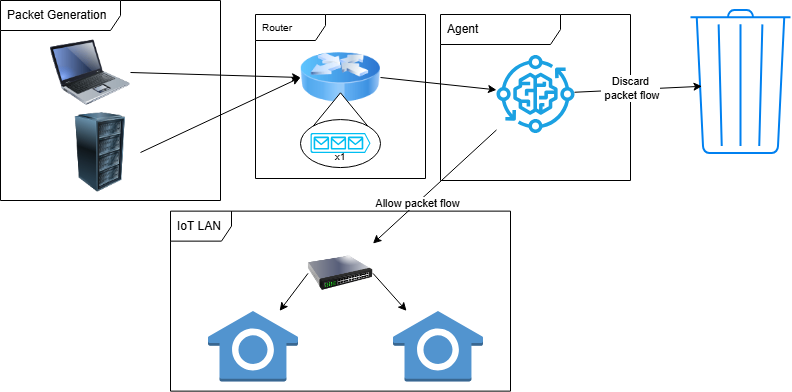
\includegraphics[width=0.9\linewidth]{RedInicial.png}
     \caption{Theoretical Environment set-up.}
     \label{fig:network-diagram}
 \end{figure}

 
\subsection{Agent Training}
 For training, the PPO Stable-Baselines3 implementation was used with a Multi-Input Policy, 200,000 time steps, and default parameters.
 Agents learn with only the information of \% of the queue occupation and discarded packets in the actual step, and have to choose between allowing or denying all traffic in the step.
\section{Experimental Results}
At this stage, the agent is trained with only DoS attacks and benign traffic.
As shown in Figure~\ref{fig:training-graph} the agent learns in response to the mean reward.
\subsection{Training Metrics}
\begin{figure}[ht]
     \centering
     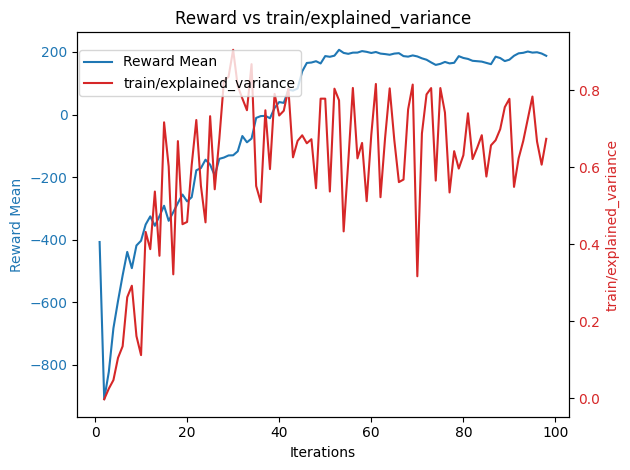
\includegraphics[width=0.60\linewidth]{output.png}
     \caption{Reward and explained variance along training.}
     \label{fig:training-graph}
 \end{figure}
The reward mean is a key metric in RL, providing insight into an agent’s performance during training. A consistent increase in the reward mean typically indicates that the agent is improving its decision making policy. Another important metric in RL is explained variance, which measures how well the model value predictions correlate with the actual rewards received. It helps identify whether the value function is learning effectively or requires further optimization, offering a quantitative measure of the model's predictive power. 
\subsection{Agent Metrics}
Figure~\ref{fig:simulation-graph} shows the behavior of the system during an attack. As the queue approaches its capacity due to the incoming attack traffic, the agent's action changes. It begins to deny packets, effectively reducing the load on the network until the attack intensity decreases and the queue stabilizes. This dynamic response illustrates how the agent adapts its decisions to mitigate the impact of DoS or DDoS attacks.
\begin{figure}[ht]
    \centering
    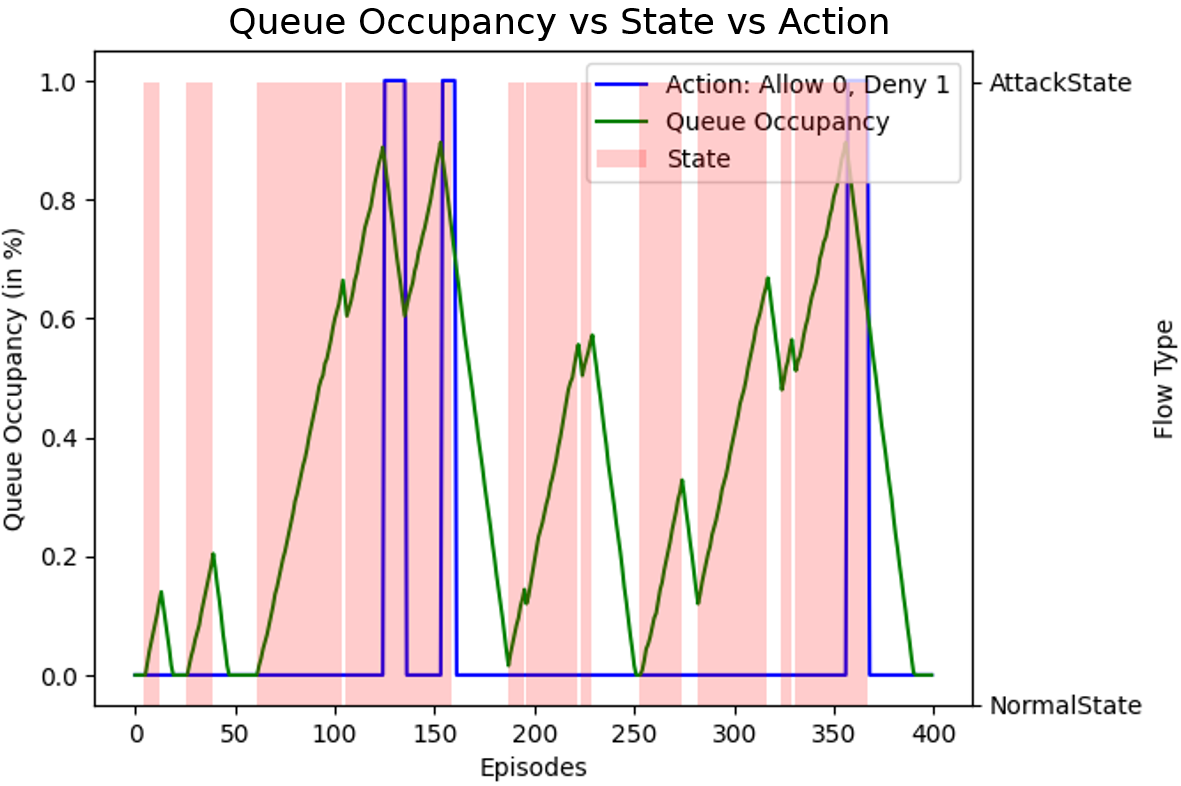
\includegraphics[width=0.75\linewidth]{RewardsActions.png}
    \caption{The queue occupation and the action in each step.}
    \label{fig:simulation-graph}
\end{figure}
\section{Conclusions and Future Work}
The increasing use of IoT devices has made them more vulnerable to cyberattacks, particularly DoS and DDoS attacks, which can severely disrupt network performance. This study demonstrates that reinforcement learning can effectively mitigate these threats by dynamically adapting to evolving attack patterns. The proposed RL-based system reduces the impact of these attacks on the local network, enhancing its stability and security.

Future work will focus on improving the adaptability of the RL agent to more sophisticated and diverse attack strategies, such as PortScan and OSScan. In addition, the expansion of the system’s capabilities to detect and mitigate other network threats will be explored.

\section*{Acknowledgments}
This publication is part of the AI4SECIoT project ("Artificial Intelligence for Securing IoT Devices"), funded by the National Cibersecurity Institute (INCIBE), derived from a collaboration agreement signed between the National Institute of Cybersecurity (INCIBE) and the University of Burgos. This initiative is carried out within the framework of the Recovery, Transformation and Resilience Plan funds, financed by the European Union (Next Generation), the project of the Government of Spain that outlines the roadmap for the modernization of the Spanish economy, the recovery of economic growth and job creation, for solid, inclusive and resilient economic reconstruction after the COVID19 crisis, and to respond to the challenges of the next decade.

 

%
% ---- Bibliography ----
%
% BibTeX users should specify bibliography style 'splncs04'.
% References will then be sorted and formatted in the correct style.
%
% \bibliographystyle{splncs04}
% \bibliography{mybibliography}
%
\bibliographystyle{splncs04}
\bibliography{references}


\end{document}
